The U-shaped curve of peak-demand-hour reduction in temperature-control-related electricity consumption is not a desirable feature of TOU electricity pricing. The fundamental intention of the time-varying tariff scheme is to reshape load profiles, especially in the peak rate period, in order to avoid excessive investment in power generation capacity. So a higher amount of reduction in electricity consumption for heating on freezing days (i.e., on days when the power grid is most burdened) serves the purpose of the price scheme. In light of that, the U-shaped evolving pattern over daily HDDs is unattractive because on days with high heating needs, TOU electricity pricing induces even less reduction in for-heating-relevant household electricity consumption. 

An alternative electricity pricing scheme, a TOU-like tariff structure with additional flexibility in price variations across daily HDDs, could address the disadvantage of typical TOU pricing revealed from my analysis (i.e., less effectiveness on days with very low temperatures). My empirical findings illustrate two important points with respect to the relationship between TOU-tariff-induced changes in household electricity consumption and price increases during the peak rate period. First, the reduction stemming from non-temperature-control-associated electricity consumption becomes larger as the magnitude of a price escalation in the peak period increases. Second, the gains obtained by marginally raising the peak-hour electricity price (i.e., an additional reduction in non-temperature-control-relevant electricity consumption) exceed the losses from such a marginal increase (i.e., a fewer reduction in temperature-control-driven electricity consumption).\footnote{See the three panels in the second column of Figure \ref{Figure:Treatment-Effects-as-a-Linear-Function-of-Price-Changes-in-the-Peak-Rate-Period}.} Those two points collectively imply that scaling up the size of a rate change in the peak rate period as daily HDDs rise enables achieving a more considerable TOU-price-induced aggregate reduction in residential electricity consumption. 

\afterpage{
    \begin{figure}[t!]
        \centering
        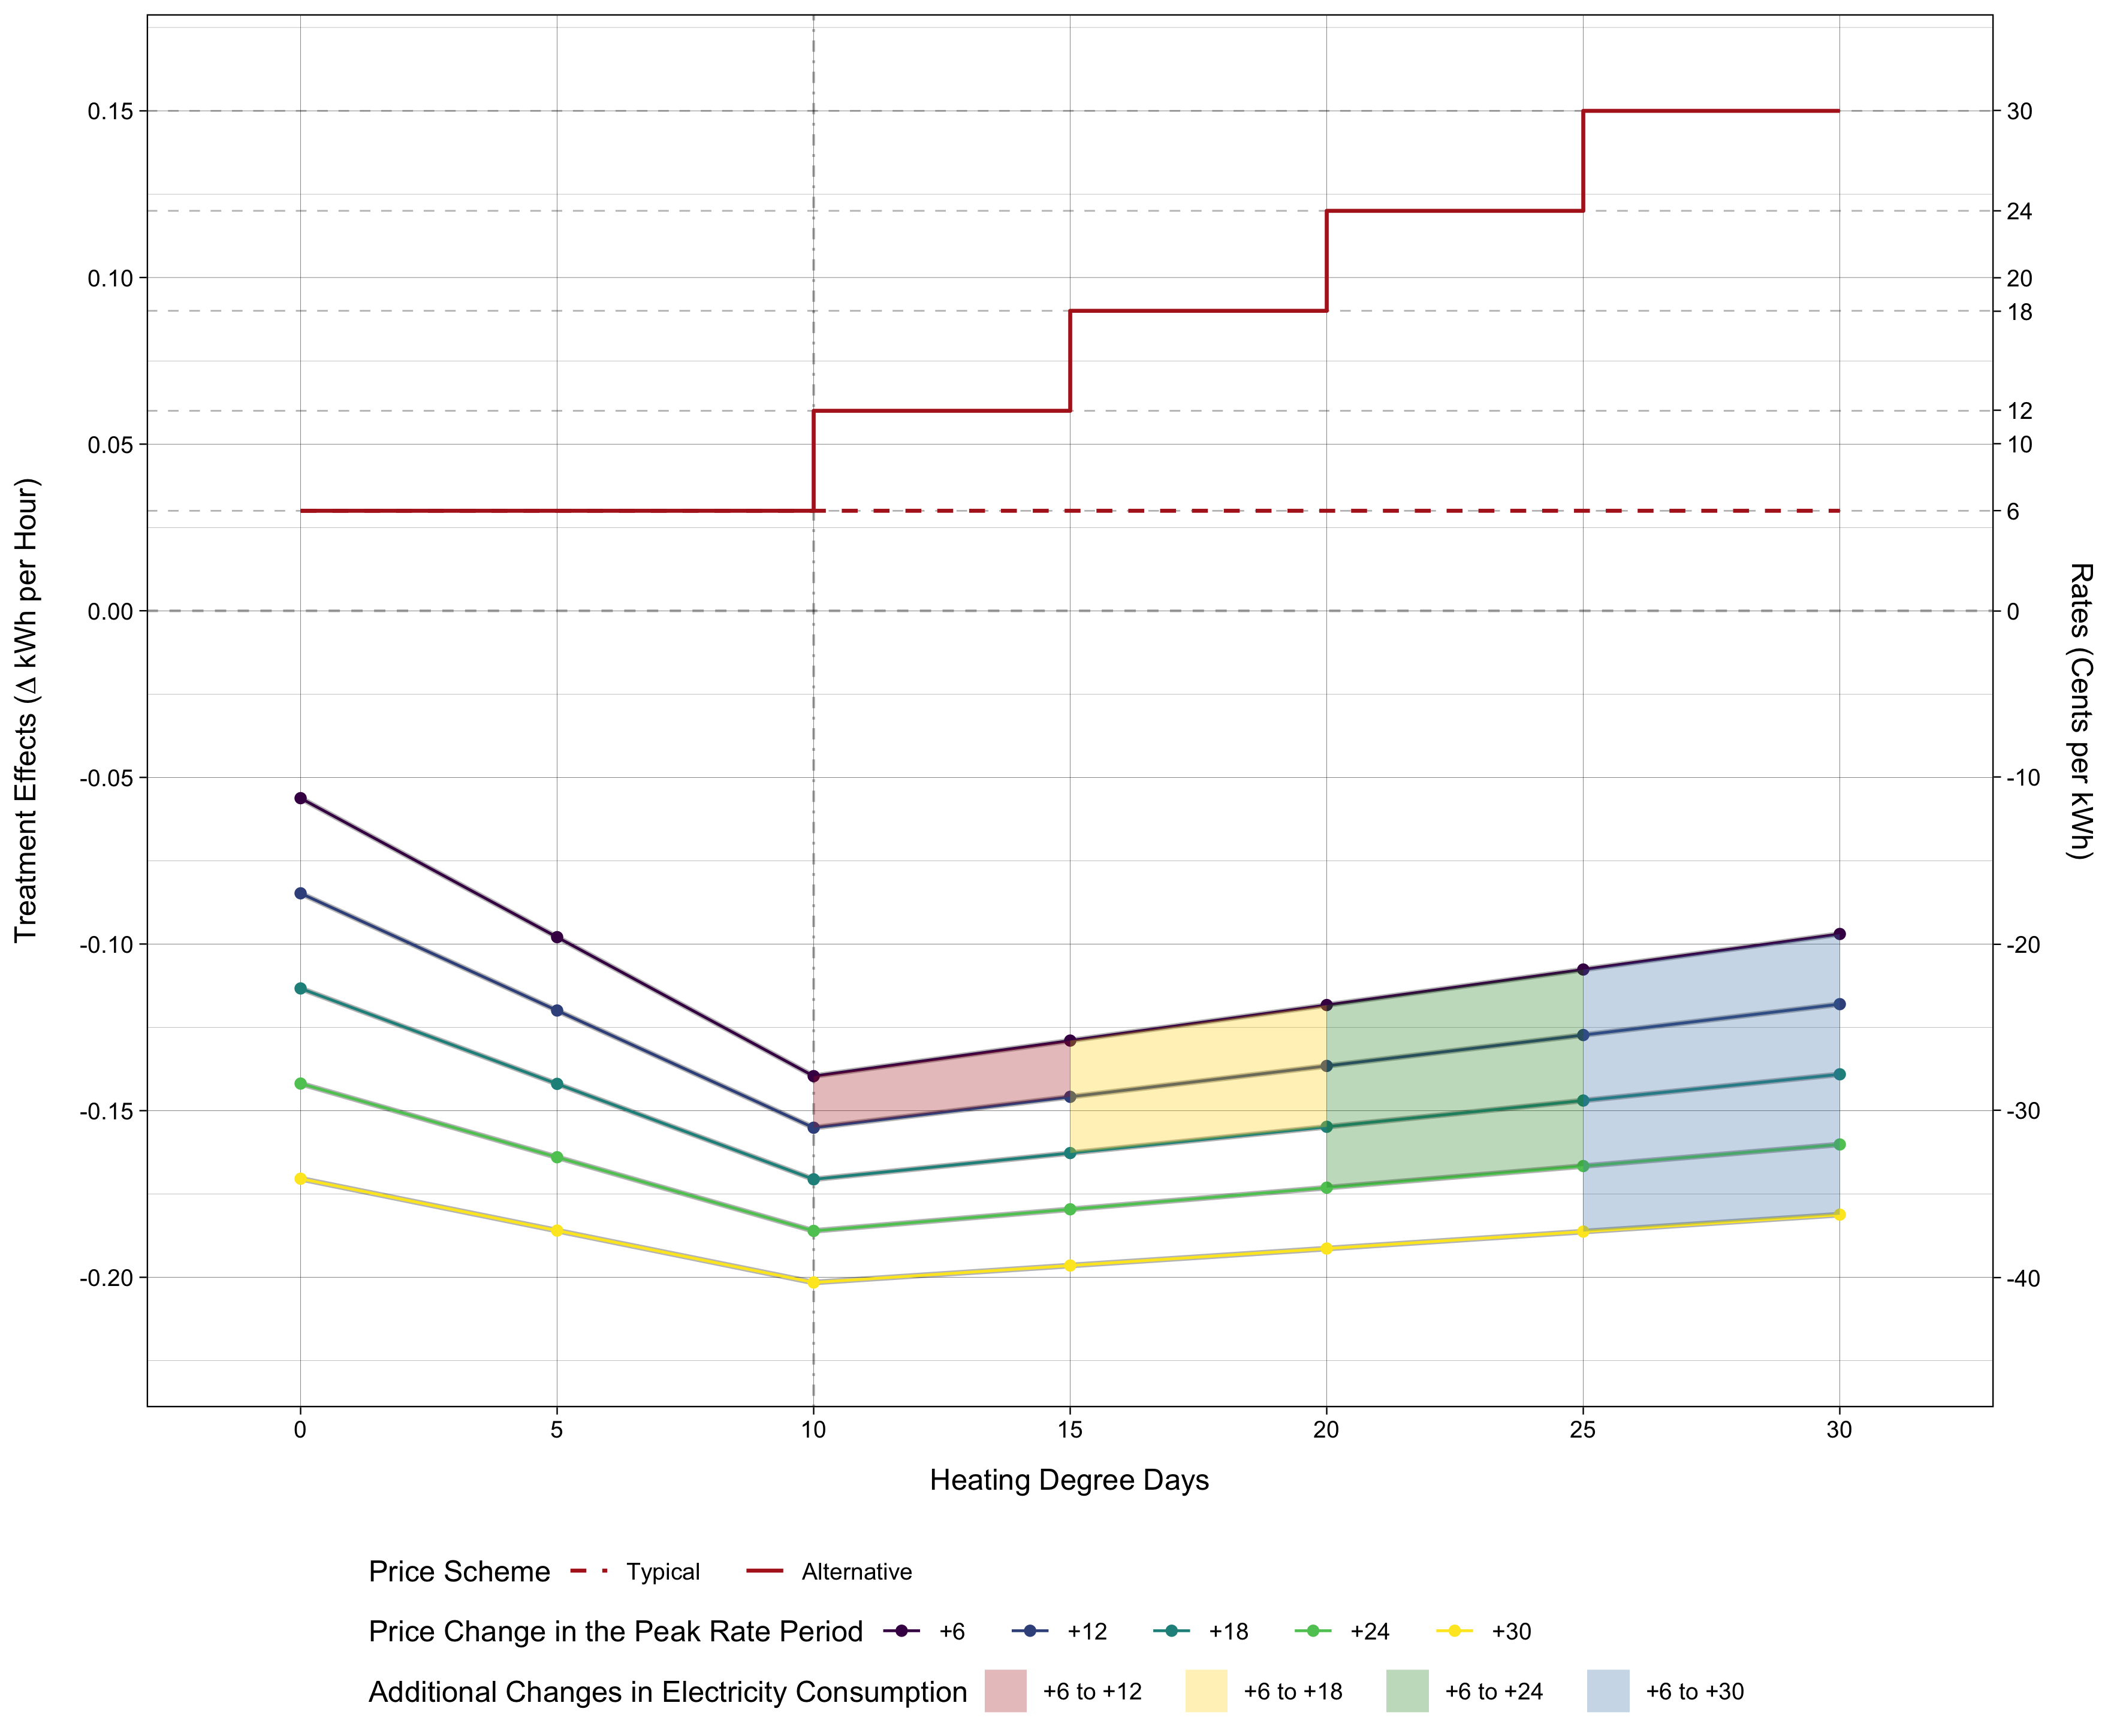
\includegraphics[scale = 0.12]{03_Chapter-2/00A_Figures/Figure_Additional-Electricity-Savings_Knot-10.png}
        \caption{Additional Gains from an Alternative Electricity Pricing Scheme}
        \caption*{
            {\small
            \textit{Note}: This figure illustrates two different price schemes. Under a typical TOU electricity pricing scheme, the rate in the peak rate period is 6 cents per $kWh$ regardless of daily HDDs. On the contrary, under an alternative tariff structure that is TOU-style but has extra flexibility across daily HDDs, the peak-hour price escalates as household heating needs grow. The shaded areas depict additional gains obtained by adopting the redesigned pricing scheme, which are mainly attributable to more significant reductions in non-temperature-control-driven household electricity consumption.
        }}
        \label{Figure:Additional-Savings-from-an-Alternative-Electricity-Pricing-Scheme}
    \end{figure}
}
Figure \ref{Figure:Additional-Savings-from-an-Alternative-Electricity-Pricing-Scheme} depicts an alternative price scheme and additional gains from it. Under the price scheme proposed in the upper part of the figure, the peak-demand-hour price jumps as household heating needs become serious. To be specific, prior to the value of daily HDDs that typical TOU pricing becomes ineffective, the magnitude of peak-rate-period price change is evenly six cents per $kWh$. After that point, every time daily HDDs rise by five, the degree of peak-demand-hour price change increases by six cents per $kWh$. 

The lower part of Figure \ref{Figure:Additional-Savings-from-an-Alternative-Electricity-Pricing-Scheme} shows additional gains from the alternative pricing scheme, which are shaded with distinct colors for each six-cent escalation in peak-rate-period price. The five U-shaped profiles over daily HDDs, indicating the predicted reductions in household electricity consumption for five different price changes in the peak rate period, are drawn by utilizing the point estimates. As illustrated in the figure, compared to the case in which the size of peak-hour price growth is fixed at six cents for all values of daily HDDs, the alternative price scheme can induce more significant reductions in household electricity consumption according to increasing household heating needs by synchronizing price increases in the peak rate period with daily HDDs. In other words, the weakness of typical TOU pricing can be alleviated under the proposed price structure. 

The alternative price scheme is well in line with the key finding in \cite{Electricity-Retail-Rate-Design-in-a-Decarbonized-Economy_Schittekatte-et-al_2022}. According to this recent paper, TOU rates complemented with Critical Peak Pricing (CPP) work well for reflecting spot-price-providing within-day load-shifting incentives. Considering that CPP introduces dramatic but short-lived price escalations when generating costs exceed a certain threshold infrequently, a very high peak price linked with exceptionally large daily HDDs in Ireland under the proposed alternative price scheme is consonant with CPP events with which TOU prices are complemented as suggested in the paper. 

In addition, this proposed price structure is better than the typical TOU tariff structure with a higher fixed peak-demand-hour price. For example, Tariff Group D reduces household electricity consumption as much as the alternative price scheme on extremely cold days. However, compared to Tariff Group D, households under the proposed price structure can consume more electricity on warm days on which the power grid still has enough spare capacity to meet higher electricity demand. 
